\documentclass[a4paper,11pt,twoside]{book}

\usepackage[english]{babel}
\usepackage{setspace}
\usepackage[utf8]{inputenc}
\usepackage{graphicx}
\usepackage{pdfpages}
\usepackage{longtable}
\usepackage{url}
\urlstyle{tt}

\usepackage{hyperref}
\usepackage{fullpage}
\usepackage{fancyhdr}

\hypersetup{
     colorlinks = true, linkcolor = blue,
     citecolor   = blue,
     urlcolor    = blue,
}


\usepackage{tocloft}
\renewcommand{\cftpartleader}{\cftdotfill{\cftdotsep}} % for parts
\renewcommand{\cftchapleader}{\cftdotfill{\cftdotsep}} % for chapters
\renewcommand{\cftsecleader}{\cftdotfill{\cftdotsep}} % for sections

\renewcommand{\headrulewidth}{0pt}

%\newcommand{\newoddpage} {\clearpage
%  \ifthenelse{\isodd{\value{page}}}{}
%  {\thispagestyle{empty}\quad\newpage}}
\thispagestyle{empty}

\newcommand{\addpaper}[5]{% #1 path; #2 label; #3 authors; #4 title; #5 URL
%  \newoddpage
  \phantomsection
  \addcontentsline{toc}{section}{#3. \emph{#4}}  

\thispagestyle{fancy} %
  
  % scriptsize / tiny
  \lfoot{\scriptsize {\tiny Nurminen, Brenner, Koponen, Latomaa, Mikhailov, Schierl, Ranasinghe, Vanmassenhove, Vidal, Aranberri, Nunziatini, Escartín, Forcada, Popovic, Scarton, Moniz (eds.)}\\
    {\tiny \em Proceedings of the 24th Annual Conference of the European Association for Machine Translation}, p. \pageref{beg#2}--\pageref{end#2}\\
      \tiny Tampere, Finland, June 2023. %\url{#5}
  }
  \cfoot{}
  %
  \label{beg#2}
  \includepdf[pages={1},pagecommand={},fitpaper=true,trim=0 0 0 0,
  offset=0 0, turn=true,noautoscale=true]{#1}
  %
  \pagestyle{fancy} %
  \lfoot{} %
  \cfoot{\thepage} 
  %
  \includepdf[pages={2-},pagecommand={\label{end#2}},fitpaper=true,trim=0 0
  0 0, offset=0 0,turn=true,noautoscale=true]{#1}
}


\newcommand{\addproject}[5]{% #1 path; #2 label; #3 authors; #4 title;
                          % #5 URL
%  \newoddpage
  \phantomsection
  \addcontentsline{toc}{section}{#3. \emph{#4}}  
  \thispagestyle{fancy} %
  \lfoot{\scriptsize {\tiny Nurminen, Brenner, Koponen, Latomaa, Mikhailov, Schierl, Ranasinghe, Vanmassenhove, Vidal, Aranberri, Nunziatini, Escartín, Forcada, Popovic, Scarton, Moniz (eds.)}\\
    {\tiny \em Proceedings of the 24th Annual Conference of the European Association for Machine Translation}, p. \pageref{beg#2}\\
      \tiny Tampere, Finland, June 2023. %\url{#5}
  }
  \cfoot{}
  %
  \label{beg#2}
  \includepdf[pages={1},pagecommand={},fitpaper=true,trim=0 0 0 0,
  offset=0 0, turn=true,noautoscale=true]{#1}
  %
  \pagestyle{fancy} %
  \lfoot{} %
  \cfoot{\thepage} 
}


\usepackage{calc}
\setlength{\footskip}{\paperheight
  -(1in+\voffset+\topmargin+\headheight+\headsep+\textheight)
  -0.6in}

\newcommand{\mychapter}[1]{
    \newpage
    \phantomsection{}
    \cfoot{}
    \vspace*{\fill}
    \begin{center}
    \begin{Huge}
    \textbf{#1}
    \end{Huge}
    \end{center}
    \addcontentsline{toc}{chapter}{#1}
    \vspace*{\fill}
    \newpage
    \cfoot{\thepage}
}

%%%%%%%%%%%%%%%%%%%%%%%%%%%%%%%%%%%%%%%%%%%%%%%%%%%%%%%%%%%%%%%828%%%%%%%%%%%%%%%%%

%\usepackage{draftwatermark}
%\SetWatermarkText{Draft}
%\SetWatermarkScale{1}

\begin{document}

\pagestyle{fancy} 
\lhead{}
\rhead{}
\chead{}
\lfoot{} 
\rfoot{} 
\cfoot{\thepage}

%\newoddpage
\thispagestyle{empty}
\enlargethispage{1cm}
\begin{center}
\phantom{x}
\vspace{-2cm}

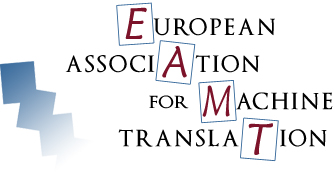
\includegraphics[width=0.8\columnwidth]{logos/eamt-logo.jpg}

\vspace{1cm}

{\huge Proceedings of the}\\[2ex]
\textbf{\huge 24th Annual Conference of \\[0.2ex]
  the European Association\\[1.0ex] for Machine Translation} 
  
\vspace{1.5cm}

{\LARGE 12 -- 15 June 2023\\
\vspace{0.5cm}
Tampere, Finland}
\vspace{3cm}

\textbf{\em Edited by}

\vspace{1em}
Mary Nurminen,
Judith Brenner,
Maarit Koponen,
Sirkku Latomaa,
Mikhail Mikhailov,
Frederike Schierl, 
Tharindu Ranasinghe,
Eva Vanmassenhove,
Sergi Alvarez Vidal,
Nora Aranberri,
Mara Nunziatini,
Carla Parra Escartín,
Mikel Forcada,
Maja Popovic,
Carolina Scarton,
Helena Moniz.

%\vspace{1cm}
\vfill

\textbf{\em Organised by}

\vspace{1em}
\begin{tabular}{ccc}

\includegraphics[width=0.35\columnwidth]{logos/tau-logo.jpg} & 
\includegraphics[width=0.30\columnwidth]{logos/uef-logo.jpg}\\
\end{tabular}
\end{center}

%\newoddpage
\thispagestyle{empty}
\vfill \mbox{} \vfill

\begin{onehalfspacing}

\noindent \includegraphics[scale=0.5]{logos/creative_commons.pdf} 
\vspace{1em}

\noindent 
The papers published in this proceedings are ---unless indicated
otherwise--- covered by the Creative Commons
Attribution-NonCommercial-NoDerivatives 4.0 International (CC-BY-NC-ND
4.0). You may copy, distribute, and transmit the work, provided that
you attribute it (authorship, proceedings, publisher) in the manner
specified by the author(s) or licensor(s), and that you do not use it
for commercial purposes. The full text of the licence may be found at
\url{https://creativecommons.org/licenses/by-nc-nd/4.0/deed.en}.

\vspace{1cm}

\noindent © 2023 The authors\\
\noindent \textbf{ISBN:} 978-952-03-2947-1\\ 
\noindent Publisher:\\
\noindent European Association for Machine Translation (EAMT)\\

\end{onehalfspacing}
\thispagestyle{empty}
\vfill \mbox{}

%%%%%%%%%%%%%%%%%%%%%%%%%%%%%%%%%%%%%%%%%%%%%%%%%%%%%%%%%%%%%%%%%%%%%%%%%%%%%%%%

%\newoddpage
\frontmatter

\tableofcontents

\begin{onehalfspacing}

\chapter*{Foreword from the General Chair}
\addcontentsline{toc}{chapter}{Foreword from the General Chair}
%\vspace{-0.8cm}
\noindent
As president of the European Association for Machine Translation (EAMT) and General Chair of the 24th Annual Conference of the EAMT, it is with great pleasure that I write these opening words to the Proceedings of EAMT 2023.\\
\\
\noindent
According to tradition, my first note of deep appreciation and gratitude goes to Heidi Depraetare and Khalil Simaan, Executive Board Members, who have moved to new adventures in their lives, after long, outstanding, and dedicated service to the EAMT community.\\
\\
\noindent
We have several milestones to celebrate this year, built upon the hard work of our Executive Committee and our community: upgraded grants for low income and war zones and for Translation Studies, a record submission rate for research projects (9 projects), a record for submissions for the best thesis candidates, and one of the highest number of papers ever submitted to our conference! I could not be prouder of the contagious energy from our community.\\
\\
\noindent
The EAMT Executive Committee (EC) has been very busy. Luc Meertens (treasurer) and Carolina Scarton (secretary) have been tirelessly supporting all initiatives. André Martins and Celia Rico, our co-chairs for low income areas, war zones and Translation Studies grants, selected 10 grantees. Barry Haddow and Carolina Scarton, our co-chairs for the Research Projects, selected 4 projects with a diverse set of topics. To all our co-chairs, my gratitude! The selection work is never an easy task and this year was particularly hard. The same applied to the best thesis award – co-chairs Carolina Scarton and Helena Moniz had a very difficult time selecting a single candidate, since the submissions were of very high quality.\\  
\\
\noindent
EAMT, as full sponsor of the MT Marathon, would also like to highlight the outstanding work that the MT Marathon organisers conducted, enriching the vitality of our community with their projects and keynotes. A special thank you to Jindra Helcl, Ond\v{r}ej Bojar, and Barry Haddow for all the efforts on yet another successful MT Marathon event.\\
\\
\noindent
EAMT, in an effort to reach out to our community in Africa, also sponsored three student grants to attend the AfricaNLP workshop at ICLR'23. Thank you, André Martins, for bridging our association with this initiative.\\
\\
\noindent
Now to Tampere, Finland! EAMT 2023 will have a three-day, four-track programme put together by our chairs: Eva Vanmassenhove and Tharindu Ranasinghe (research: technical track co-chairs); Nora Aranberri and Sergi Alvarez Vidal (research: translators \& users track co-chairs); Carla Parra Escartín and Mara Nunziatini (implementations \& case studies track co-chairs); and Mikel Forcada and Helena Moniz (products \& projects track chairs). And backing up all the scientific components of our conference and filters of quality for the final selection: our reviewers. Thank you for your work and for the alignment with all the chairs!\\ 
\\
\noindent
This year EAMT 2023 will also have an extra day for workshops and tutorials, organised by our co-chairs Judith Brenner and Maja Popovic. Once more, the submissions for workshops and tutorials largely exceeded our expectations for this inaugural year!\\ 
\\
\noindent
The programme will continue the tradition of including two keynote speakers, Lynne Bowker (Full Professor at the University of Ottawa, Canada) and Marco Turchi (Head of MT at Zoom Video Communications). Our keynote speakers will demonstrate their extensive and impactful work in Translation Studies, technologies and machine translation, speech translation, and automatic post-editing. We bring you a fresh overview of the field, integrating a wide range of topics.\\
\\
\noindent
EAMT 2023 will also include a panel on \emph{The Impact of Large Language Models (LLMs) on MT: A European View}, with several guests: Andreas Eisele (Responsible for MT at the European Union), André Martins (Unbabel/University of Lisbon), Christian Federmann (Microsoft), Helena Moniz (EAMT/University of Lisbon), Kenneth Church (Northeastern University), and Mikel Forcada (EAMT/Universitat d’Alacant). This panel is a moment to have a European view on a subject dominated by non-European initiatives.\\
\\
\noindent
EAMT 2023 would never be possible without the bright, enthusiastic, and hard working local organising team! What a dream team! Whenever EAMT had a request for a possible new addition, the answer was usually “Why not?” I’m so grateful for being able to work with you! Starting with our chair, Mary Nurminen (Tampere University), Judith Brenner (University of Eastern Finland), Maarit Koponen (University of Eastern Finland), Sirkku Latomaa (Tampere University),  Mikhail Mikhailov (Tampere University), and Frederike Schierl, (Tampere University). Thank you, Tampere University and the University of Eastern Finland, for all your support! Tampere University has been such an amazing and flexible host!\\
\\
\noindent
EAMT has been supported by generous sponsors in its initiatives along the years. This year is no exception. Our gratitude to our Silver sponsors: Pangeanic, Unbabel and ZOO Digital. To our Bronze sponsors: CrossLang, ModelFront, STAR, TransPerfect, and Welocalize. Also to Apertium, our long standing collaborator sponsor;  Springer, our Supporter sponsor for the Best Paper award; and our Media sponsors, MultiLingual and Slator. Your support is vital in our efforts to give back to our community through grants and other initiatives.\\
\\
\noindent
A note still to all our EAMT members and our participants! Without you no effort would make sense! Let us take this opportunity to create scientific collaboration and give constructive feedback. To fully enjoy the conference, please check our Code of Conduct at \url{https://events.tuni.fi/eamt23/ethics/}. I’m looking forward to seeing you all!\\ 
\\
\noindent
It is EAMT’s greatest wish to continue giving back to our community and to drive and be driven by our community’s energy and enthusiasm. Reach out to us if you have new ideas or suggestions you would like to implement. We will try hard to accomplish it with you. Learn more about us at \url{https://eamt.org/}.
\vspace{1cm}

\noindent \textbf{Helena Moniz}

\noindent President of the EAMT

\noindent General Chair of EAMT 2023

\noindent University of Lisbon / INESC-ID, Portugal

\let\cleardoublepage\clearpage

\chapter*{Message from the Organising Committee Chair}
\addcontentsline{toc}{chapter}{Message from the Organising Committee Chair}
%\vspace{-0.9cm}

\emph{Tervetuloa Tampereelle!}

\noindent 
The local organising committee welcomes you all to EAMT 2023! Thank you for choosing to join us, either in person or remotely, for 3 days of talks, posters, chats with colleagues, and evening activities. Plus an extra day for many of you to focus on a particular issue in a workshop or tutorial. Attendance at EAMT conferences continues to grow, and the highest number ever will participate in the Tampere conference.\\
\\
\noindent
After 2 conferences in the southern parts of Europe – Alacant in 2018 and (virtually) Lisbon in 2020 – EAMT moved northward to Ghent in 2022 and then farther up to Finland in 2023. Perhaps Tampere, which is on the same latitude as the southern parts of Greenland, will be the farthest north the conference will ever be held. We hope you enjoy our light nights!\\
\\
\noindent
A few new things will be introduced in this year’s conference. For the first time, we will have an extra \textbf{workshop and tutorial day} adjacent to the main conference. As first-timers, we were unsure about the number and types of proposals we would receive. We were delighted to receive a large number of proposals of very high quality, and it was difficult to make selection decisions. We hope that everyone will have a good experience with this addition to the conference!\\
\\
\noindent
A second change this year are the \textbf{conference tracks}, which have been reconfigured to show an updated view of happenings in the MT world. Whereas we previously had 1 track for research, we now have 2: one that focuses on technical research and another that focuses on academic research on translators and other types of MT users, a field that has been steadily growing. The track on implementations and case studies highlights cases of actual MT use (’in the wild’). The fourth track puts focus on various ongoing products and projects in the MT sphere.\\
\\
\noindent
The final change is that we are trying out a \textbf{hybrid light} conference attendance option to include those who cannot make it to Tampere themselves. We look forward to your feedback on all of these innovations.\\
\\
\clearpage
\noindent
A conference like this does not just happen – it is the result of great efforts by a number of people, and we’d like to thank them. First is the EAMT organisation, and especially President Helena Moniz and Secretary Carol Scarton, who went to great lengths to support our efforts. It would not have been possible without you. Next we’d like to thank our program chairs, who managed the vital work of selecting the best proposals and papers for the conference: Sergi Alvarez Vidal, Nora Aranberri, Judith Brenner, Mikel Forcada, Helena Moniz, Mara Nunziatini, Carla Parra Escartín, Maja Popovic, Tharindu Ranasinghe and Eva Vanmassenhove.\\  
\\
\noindent
We’d also like to thank our Silver sponsors, Pangeanic, Unbabel and ZOO Digital; Bronze sponsors CrossLang, ModelFront, STAR Group, TransPerfect and Welocalize; Collaborator sponsor Apertium; Supporter sponsor Springer, and Media sponsors MultiLingual and Slator. Your support of our conference and activities is greatly appreciated!\\
\\
\noindent
Thanks also go out to the Tampere University Congress Office, which made so, so much of our work easier.\\
\\
\noindent
Personally, I’d like to thank my colleagues on the local planning committee: Judith Brenner, Maarit Koponen, Sirkku Latomaa, Mikhail Mikhailov and Frederike Schierl. We have been a small but very effective, 6-person powerhouse of activity. Thank you for your enthusiasm, willingness to jump into new things, and professionalism. It has been a pleasure to serve with you.\\
\\
\noindent
We look forward to meeting you all and to your active participation in the conference! Let’s continue to make EAMT a unique space for a diverse group of researchers, developers, practitioners, leaders, vendors, users, and translators to share experiences and ideas.\\

\vspace{1cm}

\noindent \textbf{Mary Nurminen}

\noindent Tampere University and the University of Eastern Finland

\noindent On behalf of the local organising committee\\

\chapter*{Preface by the Programme Chairs}
\addcontentsline{toc}{chapter}{Preface by the Programme Chairs}

\noindent
On behalf of the programme chairs, a warm welcome to the 24th annual conference of the European Association for Machine Translation in Tampere, Finland. Following the approach which has proven so successful in the previous editions of EAMT, the conference programme consists of papers and posters divided into four tracks. However, the year 2023 sees a change in the structuring of the conference tracks. This year, we are introducing two tracks for research papers: one for more technical papers on MT development and another for research focusing on various types of users of MT. In addition to the two research tracks, two other tracks showcase use cases and implementations as well as projects and products. For the first time, the programme also includes workshops and tutorials. And the programme would not be complete without the two keynote speeches by Lynne Bowker and Marco Turchi.\\
\\
\noindent
This year at EAMT, there is a notable change since the traditional research track has been transformed into two distinct research tracks: the Technical Track and the Translators and Users Track. The \textbf{Technical Research track} invited and received technical submissions on all aspects of machine translation and related areas, serving as a hub for cutting-edge research and technological advancements, covering topics such as neural machine translation, language models, quality estimation, and more. It garnered significant attention and proved to be the most popular track at EAMT 2023, receiving a total of 51 submissions from 24 countries. Among these, 22 papers were accepted, resulting in an acceptance rate of 43\%. Seven of the accepted papers will be presented orally, while the remaining 15 will be presented as posters.\\
\\
\noindent
A considerable number of the accepted papers are centered around Neural Machine Translation (NMT) and its diverse facets. Noteworthy topics include, among others, real-word translation (Martins et al., 2023), knowledge distillation (Gumma et al., 2023), and multilingual NMT (Chichirau et al., 2023). Several papers delve into machine translation quality estimation (QE), with a specific focus on domain adaptation of QE (Sharami et al., 2023), evaluating large language models for QE (Kocmi and Federmann, 2023), and emotion translation QE (Qian et al., 2023). It was evident that leveraging large language models such as GPT and BLOOM in machine translation and related fields is a prevailing trend. Given the popularity of tools like ChatGPT, we anticipate this trend to persist in future conferences as well. Additionally, the EAMT 2023 technical research track features several papers dedicated to low-resource languages (Sannigrahi et al., 2023; Galiano-Jiménez et al., 2023).\\
\\
\noindent
Last but not least, we would like to sincerely thank all the reviewers who provided feedback and insightful comments for the submissions received. We hope you enjoy reading this year's contributions to the Technical Research Track.\\
\\
\noindent
This edition has witnessed the reshaping and renaming of the MT tracks involving users. For the first time, a research track has been assigned to showcase studies carried out from a user perspective (translators, language experts and citizens who avail of the technology without pertaining to the language industry) and properly acknowledge the value and quality of the  research in this field of study. As such, it has been the focus of the \textbf{Translators and Users Research track} to gather the widest range of topics in order to highlight the breadth of the area,  current efforts and concerns regarding the quality and use of the technology.\\
\\
\noindent
We would like to thank the response of the community, which has contributed with an extensive selection of research themes. Work spanning MT literacy, concrete use cases and guidelines for their evaluation, assessments of MT output that go beyond sentence-level precision and fluency, translation styles and editing effort were submitted to the track. We believe that their outcomes serve as feedback for MT development but also help to establish targets for researchers in this particular subfield.\\
\\
\noindent
Overall, 18 papers were submitted to the track, out of which 16 were accepted (an 89\% acceptance rate). 4 papers will be presented orally while the remaining will be exhibited in a dedicated poster session.\\
\\
\noindent
The EAMT conference has always sought to be an inclusive venue where researchers, users and MT practitioners could meet, discuss and share knowledge and expertise around machine translation from all possible points of view. With the aim of encouraging more practitioners to share their day-to-day experiences and learn from real use cases of MT, this year a new track was created: the \textbf{Implementations \& Case Studies track}. This track aims to allow those using MT in their organisations to share their experiences from different angles. The 8 papers that will be presented at the conference showcase the wide variety of topics that this may cover, from building domain-specific MT engines to using MT for epidemiological social media surveillance, among others. They all cover different domains, from e-commerce to patents, demonstrating how MT, now more than ever, is a ubiquitous technology used by very different organisations and for ever-expanding purposes. And while this happens, it still poses challenges along the way that need to be tackled in real-world settings to ensure MT implementations are successful.\\
\\
\noindent
De-la-Torre-Vilariño et al. (2023) focus on how to build a domain specific, high-quality MT workflow in the e-commerce luxury space, while Zeynep et al. (2023) experiment with how MT systems can be fine-tuned towards the specific stylistic features of literary translators for the translation of literature. Within the customer support domain, Cabeça et al. (2023) focus on building test suites to monitor MT and QE systems, paying particular attention to those errors that are critical to customers. Paulo et al. (2023) propose ways to identify context-dependent translation units that require gender agreement, and explain how to minimise such context-dependency through manipulating the translation units to make them gender-neutral and hence minimise gender bias in their MT training data. Also in the area of data preparation for MT, Wirth et al (2023) describe the process used at the European Patent Office for generating MT data to train their patent-specific MT models, and the challenges that this task poses. Chatzitheodorou et al. (2023) tackle the challenge of reconciling the competing needs of data privacy and data quality through post-editing anonymised texts. Another common challenge in MT is how to successfully incorporate terminology and tackle the tradeoffs that this may imply. Knowles et al. (2023) address this challenge in their paper. Finally, the last paper in this track explores how MT can be used for document classification purposes: Popović et al. (2023) showcase how MT can be used for scaling epidemiological social media surveillance.\\
\\
\noindent
The \textbf{Products and Projects track} has been upgraded with clearer criteria for submission, based on the extensive experience gathered after years of running this track. This year we received 20 submissions and 16 papers were accepted. The selection will provide a plethora of products and projects being developed by our community with a rich set of topics. It will surely be a very lively session with the usual poster boasters (one of our EAMT conferences’ favourite moments) and poster sessions.\\  
\\
\noindent
For the first time, this year's EAMT conference includes a \textbf{Workshop and Tutorial Day}. We invited proposals for in-depth sessions on any aspect of machine translation and related fields, and a total of 7 workshop proposals and 4 tutorial proposals were received. Almost all of the submissions were for a full-day event, demonstrating the organisers' eagerness to take the audience on a deep dive into their respective areas of expertise. After a careful review process, taking into account all aspects of the submissions, 4 workshops and 1 tutorial were accepted. The workshop topics range from gender-inclusive translation technology, open-source MT tools and automated translation of sign and spoken languages to language generation, while the tutorial explores the evolving role of the post-editor with speakers from both academia and the industry.\\
\\
\noindent
Our special thanks go to our track advisor, Jay Marciano, whose extensive experience in organising and hosting MT-related conferences and events was a great source of inspiration and guidance in the implementation of the first Workshop and Tutorial Day at an EAMT conference.\\
\\
\noindent
We also wish to thank Karen Patteri de Souza from the University of Eastern Finland for invaluable help in putting together this proceedings volume.\\

\vspace{1cm}
\begin{center}
\setlength{\tabcolsep}{20pt} 
\begin{tabular}{ll}
Nora Aranberri 		& Carla Parra Escartín\\
University of the Basque Country (UPV/EHU)	& RWS Language Weaver\\
\\
Judith Brenner			& Mikel Forcada\\
University of Eastern Finland	  & Universitat d’Alacant\\
\\ 
Maarit Koponen 		&  Maja Popovic\\
University of Eastern Finland	  & Dublin City University\\
\\
Helena Moniz			& Tharindu Ranasinghe\\ 
University of Lisbon, INESC-ID	  & University of Wolverhampton\\
\\ 
Mara Nunziatini 		& Sergi Alvarez Vidal\\
Welocalize    &  Universitat Oberta de Catalunya\\
\\
Eva Vanmassenhov\\
Tilburg University\\

\end{tabular}

\end{center}

\end{onehalfspacing}

\let\cleardoublepage\clearpage

\chapter*{EAMT 2023 Organising Committees}
\addcontentsline{toc}{chapter}{EAMT 2023 Organising Committees}

\section*{General Chair}
\noindent Helena Moniz, EAMT President, University of Lisbon, INESC-ID

\section*{Programme Chairs}
\subsection*{Research: technical track}
\noindent Tharindu Ranasinghe, University of Wolverhampton\\
\noindent Eva Vanmassenhove, Tilburg University

\subsection*{Research: translators \& users track}
\noindent Sergi Alvarez Vidal, Universitat Oberta de Catalunya\\
\noindent Nora Aranberri, University of the Basque Country (UPV/EHU)

\subsection*{Implementations \& case studies track}
\noindent Mara Nunziatini, Welocalize\\
\noindent Carla Parra Escartín, RWS Language Weaver

\subsection*{Products \& projects track}
\noindent Mikel Forcada, Universitat d’Alacant\\
\noindent Helena Moniz, University of Lisbon, INESC-ID

\subsection*{Workshops \& tutorials}
\noindent Judith Brenner, University of Eastern Finland\\
\noindent Maja Popovic, DCU

\section*{Organising committee}
\noindent Mary Nurminen, Tampere University (chair)\\
\noindent Judith Brenner, University of Eastern Finland\\
\noindent Maarit Koponen, University of Eastern Finland\\
\noindent Sirkku Latomaa, Tampere University\\
\noindent Mikhail Mikhailov, Tampere University\\
\noindent Frederike Schierl, Tampere University\\

\pagebreak

\section*{Programme Committee}
\subsection*{Research: technical track}
\noindent Fernando Alva-Manchego, Cardiff University\\
\noindent Mihael Arcan, Insight Centre for Data Analytics, National University of Ireland Galway\\
\noindent Duygu Ataman, New York University\\
\noindent Eleftherios Avramidis, German Research Center for Artificial Intelligence (DFKI)\\
\noindent Parnia Bahar, AppTek\\
\noindent Loïc Barrault, Meta AI\\
\noindent Anabela Barreiro, INESC-ID\\
\noindent Rachel Bawden, Inria\\
\noindent Luisa Bentivogli, FBK\\
\noindent Magdalena Biesialska, Universitat Politècnica de Catalunya\\
\noindent Frederic Blain, Tilburg University\\
\noindent Michael Carl, Kent State University\\
\noindent Francisco Casacuberta, Universitat Politècnica de València\\
\noindent Sheila Castilho, Dublin City University\\
\noindent Mauro Cettolo, FBK - Fondazione Bruno Kessler\\
\noindent Colin Cherry, Google\\
\noindent Vishal Chowdhary, Microsoft\\
\noindent Chenhui Chu, Kyoto University\\
\noindent Raj Dabre, IIT Bombay\\
\noindent Aswarth Abhilash Dara, Amazon Alexa AI\\
\noindent Mirella De Sisto, Tilburg University\\
\noindent Mattia Antonino Di Gangi, AppTek\\
\noindent Miguel Domingo, Universitat Politècnica de València\\
\noindent Christian Dugast, tech2biz\\
\noindent Hiroshi Echizenya, Hokkai-Gakuen University\\
\noindent Cristina España-Bonet, UdS and DFKI\\
\noindent Miquel Esplà-Gomis, Universitat d'Alacant\\
\noindent Marcello Federico, AWS AI Labs\\
\noindent Christian Federmann, Microsoft\\
\noindent Mark Fishel, University of Tartu\\
\noindent Markus Freitag, Google AI\\
\noindent Marco Gaido, Fondazione Bruno Kessler\\
\noindent Mercedes García-Martínez, Uniphore\\
\noindent Ulrich Germann, The University of Edinburgh\\
\noindent Jesús González Rubio, WebInterpret\\
\noindent Isao Goto, NHK\\
\noindent Francisco Javier Guzman, Facebook\\
\noindent Barry Haddow, The University of Edinburgh\\
\noindent Rejwanul Haque, National College of Ireland\\
\noindent Chris Hokamp, Aylien\\
\noindent Matthias Huck, SAP SE\\
\noindent Diptesh Kanojia, IIT Bombay\\
\noindent Rebecca Knowles, National Research Council Canada\\
\noindent Philipp Koehn, Johns Hopkins University\\
\noindent Shankar Kumar, Google\\
\noindent Maria Kunilovskaya, University of Saarland\\
\noindent Ekaterina Lapshinova-Koltunski, University of Hildesheim\\
\noindent Samuel Läubli, Zurich University of Applied Sciences\\
\noindent Gregor Leusch, eBay\\
\noindent Andreas Maletti, Universität Leipzig\\
\noindent Arul Menezes, Microsoft\\
\noindent Antonio Valerio Miceli Barone, Univeristy of Edinburgh\\
\noindent Helena Moniz, INESC\\
\noindent Mathias Müller, University of Zurich\\
\noindent Kenton Murray, Johns Hopkins University\\
\noindent Maria Nadejde, Amazon\\
\noindent Masaaki Nagata, NTT\\
\noindent Toshiaki Nakazawa, The University of Tokyo\\
\noindent Jan Niehues, Maastricht University\\
\noindent André Niyongabo, Princeton University\\
\noindent Constantin Orasan, University of Surrey\\
\noindent Daniel Ortiz-Martínez, Universitat de Barcelona\\
\noindent Pavel Pecina, Charles University\\
\noindent Stephan Peitz, Apple\\
\noindent Sergio Penkale, Unbabel\\
\noindent Alberto Poncelas, Rakuten Institute of Technology\\
\noindent Andrei Popescu-Belis, HEIG-VD / HES-SO\\
\noindent Maja Popovic, ADAPT Centre @ DCU\\
\noindent Preethi Raghavan, Fidelity\\
\noindent Ayla Rigouts Terryn, KU Leuven Kulak, Centre for Computational Linguistics\\
\noindent Miguel Rios, University of Vienna\\
\noindent Annette Rios Gonzales, University of Zurich\\
\noindent Rudolf Rosa, Charles University\\
\noindent Fatiha Sadat, UQAM\\
\noindent Víctor M. Sánchez-Cartagena, Universitat d'Alacant\\
\noindent Felipe Sánchez-Martínez, Universitat d'Alacant\\
\noindent Germán Sanchis-Trilles, Sciling S.L.\\
\noindent Danielle Saunders, RWS Language Weaver\\
\noindent Beatrice Savoldi, Fondazione Bruno Kessler\\
\noindent Yves Scherrer, University of Helsinki\\
\noindent Helmut Schmid, Ludwig Maximilian University of Munich\\
\noindent Rico Sennrich, University of Zurich\\
\noindent Dimitar Shterionov, Tilburg University\\
\noindent Michel Simard, National Research Council Canada (NRC)\\
\noindent Patrick Simianer, Lilt, Inc.\\
\noindent Felix Stahlberg, Google Research\\
\noindent Katsuhito Sudoh, Nara Institute of Science and Technology\\
\noindent Aleš Tamchyna, Phrase a.s.\\
\noindent Joël Tang, Imperial College London\\
\noindent Arda Tezcan, Ghent University\\
\noindent Jörg Tiedemann, University of Helsinki\\
\noindent Antonio Toral, University of Groningen\\
\noindent Masao Utiyama, NICT\\
\noindent Vincent Vandeghinste, Instituut voor de Nederlandse Taal, Leiden // Centre for Computational Linguistics, KU Leuven\\
\noindent Dušan Variš, Institute of Formal and Applied Linguistics, Charles University in Prague\\
\noindent David Vilar, Google\\
\noindent Sebastian Vincent, The University of Sheffield\\
\noindent Martin Volk, University of Zurich\\
\noindent Trang Vu, Monash University\\
\noindent Ekaterina Vylomova, The University of Melbourne\\
\noindent Longyue Wang, Tencent AI Lab\\
\noindent Taro Watanabe, Nara Institute of Science and Technology\\
\noindent Marion Weller-Di Marco, CIS - University of Munich\\
\noindent Minghao Wu, Monash University\\
\noindent Yinfei Yang, Redfin Inc.\\
\noindent François Yvon, CNRS\\
\noindent Marcos Zampieri, George mason University\\
\noindent Rabih Zbib, Avature\\
\noindent Dakun Zhang, Systran SAS

\pagebreak

\subsection*{Research: translators \& users track}
\noindent Loubna Bilali, Kent State University\\
\noindent Lynne Bowker, University of Ottawa\\
\noindent Vicent Briva-Iglesias, SFI CRT D-REAL, Dublin City University\\
\noindent Patrick Cadwell, Dublin City University\\
\noindent Michael Carl, Kent State University\\
\noindent João Lucas Cavalheiro Camargo, Dublin City University\\
\noindent Dragos Ciobanu, University of Vienna\\
\noindent Joke Daems, Ghent University\\
\noindent Helle Dam Jensen, Aarhus University\\
\noindent Alice Delorme Benites, Zurich University of Applied Sciences\\
\noindent Lettie Dorst, Leiden University\\
\noindent Emmanuelle Esperança-Rodier, LIG - GETALP - UGA\\
\noindent Maria Fernandez-Parra, Swansea University\\
\noindent Federico Gaspari, ADAPT Centre, Dublin City University\\
\noindent Ana Guerberof Arenas, University of Groningen\\
\noindent Junyan Jiang, New York University Shanghai\\
\noindent Dorothy Kenny, Dublin City University\\
\noindent Rudy Loock, Université de Lille, France, \& CNRS "Savoirs, Textes, Langage" research unit\\
\noindent Lieve Macken, Ghent University\\
\noindent Marianna Martindale, University of Maryland\\
\noindent Helena Moniz, INESC\\
\noindent Joss Moorkens, Dublin City University\\
\noindent Lucas N Vieira, University of Bristol\\
\noindent Sharon O'Brien, Dublin City University\\
\noindent Antoni Oliver, Universitat Oberta de Catalunya\\
\noindent David Orrego-Carmona, University of Warwick\\
\noindent John Ortega, Northeastern University\\
\noindent Valentina Ragni, University of Warsaw\\
\noindent Celia Rico, Universidad Complutense de Madrid\\
\noindent Alessandra Rossetti, Vrije Universiteit Brussel\\
\noindent María Del Mar Sánchez Ramos, Universidad de Alcala\\
\noindent Vilelmini Sosoni, Ionian University\\
\noindent Susana Valdez, Leiden University Centre for Linguistics

\vfill

\pagebreak

\subsubsection*{Implementations \& case studies track}
\noindent Eleftherios Avramidis, German Research Center for Artificial Intelligence (DFKI)\\
\noindent Frederick Bane, Transperfect\\
\noindent Adam Bittlingmayer, ModelFront\\
\noindent Marianna Buchicchio, Unbabel\\
\noindent Laura Casanellas, Laura Casanellas\\
\noindent Miriam Exel, SAP SE\\
\noindent Mercedes García-Martínez, Uniphore\\
\noindent László János Laki, Hungarian Research Centre for Linguistics\\
\noindent Helena Moniz, INESC\\
\noindent Raj Patel, Huawei Ireland Research Centre\\
\noindent Spyridon Pilos, European Court of Auditors\\
\noindent Heather Rossi, RWS\\
\noindent Marina Sánchez-Torrón, Unbabel\\
\noindent Konstantin Savenkov, Intento, Inc.\\
\noindent Cecilia Yalangozian, Reviewer\\
\noindent Anna Zaretskaya, TransPerfect

\vfill

\pagebreak

\subsubsection*{Products \& projects track}
\noindent Mikel Forcada, Universitat d’Alacant\\
\noindent Helena Moniz, University of Lisbon (FLUL), INESC-ID

\clearpage

\subsection*{Thesis award}
\noindent Rachel Bawden, Inria\\
\noindent Daniel Beck, The University of Melbourne\\
\noindent William Byrne, University of Cambridge\\
\noindent José G. C. de Souza, Unbabel\\
\noindent Vera Cabarrão, Unbabel / INESC-ID\\
\noindent Sheila Castilho, Dublin City University\\
\noindent Anna Currey, Amazon Web Services\\
\noindent Mattia Antonino Di Gangi, AppTek\\
\noindent Maha Elbayad, LIG/ Inria\\
\noindent Miquel Esplà-Gomis, Universitat d'Alacant\\
\noindent Marcello Federico, Amazon AI\\
\noindent Mikel Forcada, DLSI - Universitat d'Alacant\\
\noindent Barry Haddow, The University of Edinburgh\\
\noindent Diptesh Kanojia, IIT Bombay\\
\noindent Philipp Koehn, Johns Hopkins University\\
\noindent Helena Moniz, INESC/FLUL\\
\noindent Mary Nurminen, Tampere University\\
\noindent Constantin Orasan, University of Surrey\\
\noindent John E. Ortega, Northeastern University\\
\noindent Santanu Pal, Wipro Limited\\
\noindent Pavel Pecina, Charles University\\
\noindent Maja Popovic, ADAPT Centre @ DCU\\
\noindent Celia Rico, Universidad Complutense de Madrid\\
\noindent Víctor M. Sánchez-Cartagena, Universitat d'Alacant\\
\noindent Marina Sánchez-Torrón, Unbabel\\
\noindent Danielle Saunders, University of Cambridge\\
\noindent Dimitar Shterionov, Tilburg University\\
\noindent Felix Stahlberg, Google Research\\
\noindent Arda Tezcan, Ghent University\\
\noindent Antonio Toral, University of Groningen\\
\noindent Ualsher Tukeyev, al-Farabi Kazakh National University\\
\noindent Bram Vanroy, KU Leuven; Ghent University\\
\noindent Longyue Wang, Tencent AI Lab\\

%\newoddpage
\mainmatter

\chapter*{Keynote Addresses}
\addcontentsline{toc}{chapter}{Keynote Addresses}
\section*{Towards an Outward Turn in Translation Technology Research?}\label{invited}
\textbf{Lynne Bowker}, University of Ottawa
\vspace{0.5cm}

\begin{onehalfspacing}
\noindent
In 2019, Susan Bassnett and David Johnson guest edited a special issue of \emph{The Translator} (vol. 25, issue 3) with the theme “the Outward Turn”. In the introduction, the editors note that Translation Studies (TS) has witnessed numerous turns in the past decades (e.g. linguistic, cultural, sociological), and is perhaps not really in need of another, not the least because fields do not develop in a neat linear way. Nevertheless, Bassnett and Johnson point to what they see as a potentially worrying trend whereby TS scholars seem increasingly to talk mainly to one another, which puts TS at risk of lurching “into ultimate self-referentiality, especially in the global academic marketplace where reference and citation are perceived as valuable ends in themselves” (p. 185). Of course, the fields of translation technology and TS do not face precisely the same issues, nor will they necessarily benefit from the same specific approaches. Yet at a higher level, we might do well to pay attention to discussions about an Outward Turn in TS and consider how this could benefit the translation technology community. For instance, Bassnett and Johnson suggest that at one level, the idea of an Outward Turn entails the recognition of the need for an increasing plurality of voices from across the globe; yet, this must be coupled with a recognition of the importance of creating space where different traditions can maintain their perspective and assert the value of their own concerns and insights within the homogenizing context of internationalization. In other words, an Outward Turn in TS would see researchers focus on the issues that increasingly surround them and recognize that uniformity can ultimately be damaging for everyone. In what ways might the broad strokes of an Outward Turn be relevant for translation technology research? This presentation will consider how various aspects of this need for expanding horizons within and beyond the contours of the translation technology field could manifest themselves in our collective research agenda.\\
\end{onehalfspacing}
\vfill 
\clearpage

\section*{Towards Real-time Meeting Translation}\label{invited}
\textbf{Marco Turchi}, Zoom Video Communications
\vspace{0.5cm}

\begin{onehalfspacing}
\noindent
Nowadays, machine translation (MT) has become the prominent solution to break language barriers and is used daily to translate emails, chats, technical documents, news articles, etc. At Zoom, we provide users with translation solutions to allow them to better connect, collaborate, and communicate in different languages during meetings. However, different from the classic speech translation use cases including TED talks or European Parliament sessions, the meeting scenario poses several challenges for MT technology. For instance, when speaking spontaneously, people introduce hesitations and repetitions, and, when interacting with other participants, they generate truncated, overlapped, and malformed utterances. So, in addition to the speech recognition errors, the MT system needs to simultaneously deal with all these factors to generate the optimal translation in real time. In my presentation, I will initially focus on highlighting the main challenges of meeting translation, paying attention to those phenomena that have a critical impact on the final output. Then, I will present some solutions that can be used to mitigate these problems and enhance translation quality in meetings.\\
\end{onehalfspacing}
\vspace{1cm}

\chapter*{EAMT 2023 Best Thesis Award --- Anthony C Clarke Award}
\addcontentsline{toc}{chapter}{EAMT 2023 Best Thesis Award --- Anthony C Clarke Award}

\begin{onehalfspacing}

\noindent
Nine PhD theses defended in 2022 were received as candidates for the 2022 edition of the EAMT Best Thesis Award, and all nine were eligible. 28 reviewers and 6 EAMT Executive Committee members were recruited to examine and score the theses, considering how challenging the problem tackled in each thesis was, how relevant the results were for machine translation as a field, and what the strength of its impact in terms of scientific publications was. Two EAMT Executive Committee members also analysed all theses. It became very clear that 2022 was another very good year for PhD theses in machine translation.\\ 
\\
\noindent
All theses had merit, all candidates had strong CVs and, therefore, it was very difficult to select a winner.\\
\\
\noindent
A panel of two EAMT Executive Committee members (Carolina Scarton and Helena Moniz) was assembled to process the reviews and select a winner that was later ratified by the EAMT executive committee.\\
\\
\noindent
We are pleased to announce that the awardee of the 2022 edition of the EAMT Best Thesis is \textbf{Biao Zhang's thesis "Towards Efficient Universal Neural Machine Translation"} (University of Edinburgh, UK), supervised by Dr Rico Sennrich and Dr Ivan Titov.\\
\\
\noindent
The awardee will receive a prize of €500, together with a suitably-inscribed certificate. In addition, Dr. Zhang will present a summary of their thesis at the 24rd Annual Conference of the European Association for Machine Translation (EAMT 2023: \url{https://events.tuni.fi/eamt23/}) which will take place from June 12th to 15th in Tampere, Finland. In order to facilitate this, the EAMT will waive the winner's registration costs and will make available a travel bursary of €200.\\  

\end{onehalfspacing}

\vspace{1cm}

\noindent Helena Moniz, EAMT President

\noindent Carolina Scarton, EAMT Secretary

\newpage
\addpaper{misc/EAMT_Best_Thesis_Abstract.pdf}{btaw}{Biao Zhang}{Towards Efficient Universal Neural Machine Translation}{}

\mychapter{Research: Technical}

\addpaper{papers_restech/EAMT_2023_paper_538.pdf}{pr538}{Javad Pourmostafa Roshan Sharami, Dimitar Shterionov, Frédéric Blain, Eva}{Tailoring Domain Adaptation for Machine Translation Quality Estimation}{}
\addpaper{papers_restech/EAMT_2023_paper_862.pdf}{pr862}{Elise Bertin-Lemée, Annelies Braffort, Camille Challant, Claire Danet and Michael Filhol}{Example-Based Machine Translation from Textto a Hierarchical Representation of Sign Language}{}
\addpaper{papers_restech/EAMT_2023_paper_913.pdf}{pr913}{Mikko Aulamo, Ona de Gibert, Sami Virpioja and Jörg Tiedemann}{Unsupervised Feature Selection for Effective Parallel Corpus Filtering}{}
\addpaper{papers_restech/EAMT_2023_paper_1299.pdf}{pr1299}{Antoni Oliver González and Sergi Álvarez}{Filtering and rescoring the CCMatrix corpus for Neural Machine Translation training}{}
\addpaper{papers_restech/EAMT_2023_paper_1564.pdf}{pr1564}{Taisiya Glushkova, Chrysoula Zerva and André F. T. Martins}{BLEU Meets COMET: Combining Lexical and Neural Metrics Towards Robust Machine Translation Evaluation}{}
\addpaper{papers_restech/EAMT_2023_paper_2510.pdf}{pr2510}{Aarón Galiano-Jiménez, Felipe Sánchez-Martínez, Víctor M. Sánchez-Cartagena and Juan Antonio Pérez-Ortiz}{Exploiting large pre-trained models for low-resource neural machine translation}{}
\addpaper{papers_restech/EAMT_2023_paper_3498.pdf}{pr3498}{Nathaniel Berger, Miriam Exel, Matthias Huck and Stefan Riezler}{Enhancing Supervised Learning with Contrastive Markings in Neural Machine Translation Training}{}
\addpaper{papers_restech/EAMT_2023_paper_3997.pdf}{pr3997}{Francesco Fernicola, Silvia Bernardini, Federico Garcea, Adriano Ferraresi and Alberto Barrón-Cedeño}{Return to the Source: Assessing Machine Translation Suitability}{}
\addpaper{papers_restech/EAMT_2023_paper_5483.pdf}{pr5483}{Jianfei He, Shichao Sun, Xiaohua Jia and Wenjie Li}{Empirical Analysis of Beam Search Curse and Search Errors with Model Errors in Neural Machine Translation}{}
\addpaper{papers_restech/EAMT_2023_paper_5627.pdf}{pr5627}{Varun Gumma, Raj Dabre and Pratyush Kumar}{An Empirical Study of Leveraging Knowledge Distillation for Compressing Multilingual Neural Machine Translation Models}{}
\addpaper{papers_restech/EAMT_2023_paper_6052.pdf}{pr6052}{Pedro Henrique Martins, João Alves, Tânia Vaz, Madalena Gonçalves, Beatriz Silva, Marianna Buchicchio, José G. C. de Souza and André F. T. Martins}{Empirical Assessment of kNN-MT for Real-World Translation Scenarios}{}
\addpaper{papers_restech/EAMT_2023_paper_6097.pdf}{pr6097}{Shenbin Qian, Constantin Orasan, Felix Do Carmo, Qiuliang Li and Diptesh Kanojia}{Evaluation of Chinese-English Machine Translation of Emotion-Loaded Microblog Texts: A Human Annotated Dataset for the Quality Assessment of Emotion Translation}{}
\addpaper{papers_restech/EAMT_2023_paper_6201.pdf}{pr6201}{Benoist Wolleb, Romain Silvestri, Georgios Vernikos, Ljiljana Dolamic and Andrei Popescu-Belis}{Assessing the Importance of Frequency versus Compositionality for Subword-based Tokenization in NMT}{}
\addpaper{papers_restech/EAMT_2023_paper_6801.pdf}{pr6801}{Harritxu Gete, Thierry Etchegoyhen and Gorka Labaka}{What Works When in Context-aware Neural Machine Translation?}{}
\addpaper{papers_restech/EAMT_2023_paper_6819.pdf}{pr6819}{Rachel Bawden and François Yvon}{Investigating the Translation Performance of a Large Multilingual Language Model: the Case of BLOOM}{}
\addpaper{papers_restech/EAMT_2023_paper_7058.pdf}{pr7058}{Flavia De Camillis, Egon W. Stemle, Elena Chiocchetti and Francesco Fernicola}{The MT@BZ corpus: machine translation \& legal language}{}
\addpaper{papers_restech/EAMT_2023_paper_7558.pdf}{pr7558}{Sonal Sannigrahi and Rachel Bawden}{Investigating Lexical Sharing in Multilingual Machine Translation for Indian Languages}{}
\addpaper{papers_restech/EAMT_2023_paper_7632.pdf}{pr7632}{Tom Kocmi and Christian Federmann}{Large Language Models Are State-of-the-Art Evaluators of Translation Quality}{}
\addpaper{papers_restech/EAMT_2023_paper_7919.pdf}{pr7919}{Ali Vardasbi, Telmo Pessoa Pires, Robin Schmidt and Stephan Peitz}{State Spaces Aren't Enough: Machine Translation Needs Attention}{}
\addpaper{papers_restech/EAMT_2023_paper_8587.pdf}{pr8587}{Malina Chichirau, Rik van Noord and Antonio Toral}{Automatic Discrimination of Human and Neural Machine Translation in Multilingual Scenarios}{}
\addpaper{papers_restech/EAMT_2023_paper_9340.pdf}{pr9340}{Yasmin Moslem, Rejwanul Haque, John D. Kelleher and Andy Way}{Adaptive Machine Translation with Large Language Models}{}
\addpaper{papers_restech/EAMT_2023_paper_9634.pdf}{pr9634}{Angel Navarro, Miguel Domingo and Francisco Casacuberta}{Segment-based Interactive Machine Translation at a Character Level}{}

\mychapter{Research: Translators and users}

\addpaper{papers_restrans/EAMT_2023_paper_948.pdf}{ptu948}{Manuel Lardelli and Dagmar Gromann}{Gender-Fair Post-Editing: A Case Study Beyond the Binary}{}
\addpaper{papers_restrans/EAMT_2023_paper_1842.pdf}{ptu1842}{Miguel A. Jimenez-Crespo}{“Translationese” (and “post-editese”?) no more: on importing fuzzy conceptual tools from Translation Studies in MT research}{}
\addpaper{papers_restrans/EAMT_2023_paper_2278.pdf}{ptu2278}{María Do Campo Bayón and Pilar Sánchez-Gijón}{A social media NMT engine for a low-resource language combination}{}
\addpaper{papers_restrans/EAMT_2023_paper_2411.pdf}{ptu2411}{Hadeel Saadany, Constantin Orasan, Rocio Caro Quintana, Felix Do Carmo and Leonardo Zilio}{Analysing Mistranslation of Emotions in \textbackslash\textbackslash Multilingual Tweets by Online MT Tools}{}
\addpaper{papers_restrans/EAMT_2023_paper_3299.pdf}{ptu3299}{Janiça Hackenbuchner and Ralph Krüger}{DataLitMT – Teaching Data Literacy in the Context of Machine Translation Literacy}{}
\addpaper{papers_restrans/EAMT_2023_paper_3934.pdf}{ptu3934}{Salmi Leena, Aletta G. Dorst, Maarit Koponen and Katinka Zeven}{Do Humans Translate like Machines? Students’ Conceptualisations of Human and Machine Translation}{}
\addpaper{papers_restrans/EAMT_2023_paper_4057.pdf}{ptu4057}{Lieve Macken, Bram Vanroy and Arda Tezcan}{Adapting Machine Translation Education to the Neural Era: A Case Study of MT Quality Assessment}{}
\addpaper{papers_restrans/EAMT_2023_paper_4761.pdf}{ptu4761}{Sergi Alvarez and Antoni Oliver}{PE effort and neural-based automatic MT metrics: do they correlate?}{}
\addpaper{papers_restrans/EAMT_2023_paper_4957.pdf}{ptu4957}{Susana Valdez, Ana Guerberof Arenas and Kars Ligtenberg}{Migrant communities living in the Netherlands and their use of MT in healthcare settings}{}
\addpaper{papers_restrans/EAMT_2023_paper_5396.pdf}{ptu5396}{Vicent Briva-Iglesias and Sharon O'Brien}{Measuring Machine Translation User Experience (MTUX): A Comparison between AttrakDiff and User Experience Questionnaire}{}
\addpaper{papers_restrans/EAMT_2023_paper_6805.pdf}{ptu6805}{Fred Bane, Anna Zaretskaya, Tània Blanch Miró, Celia Soler Uguet and João Torres}{Coming to Terms with Glossary Enforcement: A Study of Three Approaches to Enforcing Terminology in NMT}{}
\addpaper{papers_restrans/EAMT_2023_paper_7589.pdf}{ptu7589}{Miguel Angel Rios Gaona, Raluca-Maria Chereji, Alina Secara and Dragos Ciobanu}{Quality Analysis of Multilingual Neural Machine Translation Systems and Reference Test Translations for the English-Romanian language pair in the Medical Domain}{}
\addpaper{papers_restrans/EAMT_2023_paper_7680.pdf}{ptu7680}{Maja Popovic, Ekaterina Lapshinova-Koltunski and Maarit Koponen}{Computational analysis of different translations: by professionals, students and machines}{}
\addpaper{papers_restrans/EAMT_2023_paper_8995.pdf}{ptu8995}{Bettina Hiebl and Dagmar Gromann}{Quality in Human and Machine Translation: An Interdisciplinary Survey}{}
\addpaper{papers_restrans/EAMT_2023_paper_9159.pdf}{ptu9159}{Fadi Al-Ghawanmeh, Alexander Jensenius and Kamel Smaili}{How can machine translation help generate Arab melodic improvisation?}{}
\addpaper{papers_restrans/EAMT_2023_paper_9777.pdf}{ptu9777}{Sheila Castilho, Clodagh Quinn Mallon, Rahel Meister and Shengya Yue}{Do online Machine Translation Systems Care for Context? What About a  GPT Model?}{}

\mychapter{Implementations and case studies}

\addpaper{papers_implement/EAMT_2023_paper_3537.pdf}{pi3537}{Zeynep Yirmibeşoğlu, Olgun Dursun, Harun Dallı, Mehmet Şahin, Ena Hodzik, Sabri Gürses and Tunga Güngör}{Incorporating Human Translator Style into English-Turkish Literary Machine Translation}{}
\addpaper{papers_implement/EAMT_2023_paper_4282.pdf}{pi4282}{Konstantinos Chatzitheodorou, M.ª Ángeles García Escrivá and Carmen Grau Lacal}{Machine translation of anonymized documents with human-in-the-loop}{}
\addpaper{papers_implement/EAMT_2023_paper_6949.pdf}{pi6949}{Marjolene Paulo, Vera Cabarrão, Helena Moniz, Miguel Menezes, Rachel Grewcock and Eduardo Farah}{Context-aware and gender-neutral Translation Memories}{}
\addpaper{papers_implement/EAMT_2023_paper_7464.pdf}{pi7464}{Jose-Manuel De-la-Torre-Vilariño, Juan-Luis García-Mendoza and Alessia Petrucci}{Improving Machine Translation in the E-commerce Luxury Space. A case study}{}
\addpaper{papers_implement/EAMT_2023_paper_8264.pdf}{pi8264}{Mariana Cabeça, Marianna Buchicchio, Madalena Gonçalves, Christine Maroti, João Godinho, Pedro Coelho, Helena Moniz and Alon Lavie}{Quality Fit for Purpose: Building Business Critical Errors Test Suites}{}
\addpaper{papers_implement/EAMT_2023_paper_9005.pdf}{pi9005}{Maja Popovic, Vasudevan Nedumpozhimana, Meegan Gower, Sneha Rautmare, Nishtha Jain and John Kelleher}{Using MT for multilingual covid-19 case load prediction from social media texts}{}
\addpaper{papers_implement/EAMT_2023_paper_9046.pdf}{pi9046}{Matthias Wirth, Volker D. Hähnke, Franco Mascia, Arnaud Wéry, Konrad Vowinckel, Marco del Rey, Raúl Mohedano del Pozo, Pau Montes and Alexander Klenner-Bajaja}{Building Machine Translation Tools for Patent Language: A Data Generation Strategy at the European Patent Office}{}
\addpaper{papers_implement/EAMT_2023_paper_9943.pdf}{pi9943}{Rebecca Knowles, Samuel Larkin, Marc Tessier and Michel Simard}{Terminology in Neural Machine Translation: A Case Study of the Canadian Hansard}{}

\mychapter{Products and projects}

\addpaper{papers_prodproj/EAMT_2023_paper_103.pdf}{pp103}{Paola Ruffo, Joke Daems and Lieve Macken}{Developing User-centred Approaches to Technological Innovation in Literary Translation (DUAL-T)}{}
\addpaper{papers_prodproj/EAMT_2023_paper_212.pdf}{pp212}{Marie-Aude Lefer, Romane Bodart, Adam Obrusnik and Justine Piette}{The Post-Edit Me! project}{}
\addpaper{papers_prodproj/EAMT_2023_paper_1245.pdf}{pp1245}{Antoni Oliver, Mercè Vàzquez, Marta Coll-Florit, Sergi Álvarez, Víctor Suárez, Claudi Aventín-Boya, Cristina Valdés, Mar Font and Alejandro Pardos}{TAN-IBE: Neural Machine Translation for the romance languages of the Iberian Peninsula}{}
\addpaper{papers_prodproj/EAMT_2023_paper_1994.pdf}{pp1994}{Cristina Toledo Báez}{GAMETRAPP: Training app for post-editing neural machine trans-lation using gamification in professional settings}{}
\addpaper{papers_prodproj/EAMT_2023_paper_2945.pdf}{pp2945}{Bram Vanroy, Arda Tezcan and Lieve Macken}{MATEO: MAchine Translation Evaluation Online}{}
\addpaper{papers_prodproj/EAMT_2023_paper_2986.pdf}{pp2986}{Vincent Vandeghinste, Dimitar Shterionov, Mirella De Sisto, Aoife Brady, Mathieu De Coster, Lorraine Leeson, Josep Blat, Frankie Picron, Marcello Paolo Scipioni, Aditya Parikh, Louis ten Bosch, John O'Flaherty, Joni Dambre, Jorn Rijckaert, Bram Vanroy, Victor Ubieto Nogales, Santiago Egea Gomez, Ineke Schuurman, Gorka Labaka, Adrián Núñez-Marcos, Irene Murtagh, Euan McGill and Horacio Saggion}{SignON: Sign Language Translation. Progress and challenges.}{}
\addpaper{papers_prodproj/EAMT_2023_paper_4844.pdf}{pp4844}{Mirella De Sisto, Vincent Vandeghinste, Lien Soetemans, Caro Brosens and Dimitar Shterionov}{GoSt-ParC-Sign: Gold Standard Parallel Corpus of Sign and spoken language}{}
\addpaper{papers_prodproj/EAMT_2023_paper_5012.pdf}{pp5012}{Marta Bañón, Mălina Chichirău, Miquel Esplà-Gomis, Mikel Forcada, Aarón Galiano-Jiménez, Taja Kuzman, Nikola Ljubešić, Rik van Noord, Leopoldo Pla Sempere, Gema Ramírez-Sánchez, Peter Rupnik, Vit Suchomel, Antonio Toral and Jaume Zaragoza-Bernabeu}{MaCoCu: Massive collection and curation of monolingual and bilingual data: focus on under-resourced languages}{}
\addpaper{papers_prodproj/EAMT_2023_paper_5081.pdf}{pp5081}{Mathias Müller, Sarah Ebling, Eleftherios Avramidis, Alessia Battisti, Michèle Berger, Richard Bowden, Annelies Braffort, Necati Cihan Camgoz, Cristina España-Bonet, Roman Grundkiewicz, Zifan Jiang, Oscar Koller, Amit Moryossef, Regula Perrollaz, Sabine Reinhard, Annette Rios Gonzales, Dimitar Shterionov, Sandra Sidler-Miserez, Katja Tissi and Davy Van Landuyt}{First WMT Shared Task on Sign Language Translation (WMT-SLT22)}{}
\addpaper{papers_prodproj/EAMT_2023_paper_5246.pdf}{pp5246}{Maarit Koponen, Mary Nurminen, Nina Havumetsä and Juha Lång}{DECA: Democratic epistemic capacities in the age of algorithms}{}
\addpaper{papers_prodproj/EAMT_2023_paper_5533.pdf}{pp5533}{Yves Scherrer, Olli Kuparinen and Aleksandra Miletic}{CorCoDial - Machine translation techniques for corpus-based computational dialectology}{}
\addpaper{papers_prodproj/EAMT_2023_paper_5543.pdf}{pp5543}{Julian Hamm and Judith Klein}{How STAR Transit NXT can help translators measure and increase their MT post-editing efficiency}{}
\addpaper{papers_prodproj/EAMT_2023_paper_7877.pdf}{pp7877}{Lucía Ormaechea, Pierrette Bouillon, Maximin Coavoux, Emmanuelle Esperança-Rodier, Johanna Gerlach, Jerôme Goulian, Benjamin Lecouteux, Cécile Macaire, Jonathan Mutal, Magali Norré, Adrien Pupier and Didier Schwab}{PROPICTO: Developing Speech-to-Pictograph Translation Systems to Enhance Communication Accessibility}{}
\addpaper{papers_prodproj/EAMT_2023_paper_9781.pdf}{pp9781}{Mikko Aulamo, Nikolay Bogoychev, Shaoxiong Ji, Graeme Nail, Gema Ramírez-Sánchez, Jörg Tiedemann, Jelmer van der Linde and Jaume Zaragoza}{HPLT: High Performance Language Technologies}{}

%\newpage
%\cfoot{}
%\phantom{x}
\let\cleardoublepage\clearpage

\chapter*{Sponsors}
\addcontentsline{toc}{chapter}{Sponsors}

% Add logos here
\section*{Silver sponsors}

\vfill

\begin{center}

\includegraphics[width=0.6\columnwidth]{logos/pangeanic-logo.png}

\vfill


\includegraphics[width=0.6\columnwidth]{logos/unbabel-logo.png}

\vfill


\includegraphics[width=0.6\columnwidth]{logos/zoo-logo.jpg}
\end{center}
\thispagestyle{empty}
\vfill

\newpage

\section*{Bronze sponsors}


\includegraphics[width=0.40\columnwidth]{logos/crosslang-logo.png} \hfill
\vfill
\hfill 
\includegraphics[width=0.40\columnwidth]{logos/modelfront-logo.png} 
\vfill

\includegraphics[width=0.40\columnwidth]{logos/star-logo.png} \hfill
\vfill
\hfill 
\includegraphics[width=0.40\columnwidth]{logos/global-link.jpg} 
\vfill

\includegraphics[width=0.40\columnwidth]{logos/welocalize-logo.png}  \hfill
\vfill
\thispagestyle{empty}

\newpage

\section*{Collaborators}
\begin{center}

\includegraphics[width=0.5\columnwidth]{logos/apertium-logo.jpg}
\end{center}

\vfill

\section*{Supporters}

\begin{center}

\includegraphics[width=0.55\columnwidth]{logos/springer-logo.png}
\end{center}

\vfill

\section*{Media sponsors}

\begin{center}

\includegraphics[width=0.6\columnwidth]{logos/multilingual-logo.png}

\vfill


\includegraphics[width=0.6\columnwidth]{logos/slator-logo.png}
\thispagestyle{empty}
\end{center}

\vfill

\section*{Institutional partners}

\begin{center}
\vfill

\includegraphics[width=0.6\columnwidth]{logos/tau-logo.jpg}\\
\vfill

\includegraphics[width=0.6\columnwidth]{logos/uef-logo.jpg}
\vfill
\end{center}
\thispagestyle{empty}

\end{document}
